\section{Force Systems}

\subsection{Equivalent systems}

\blue{Do we need this section?}

It can be helpful at times to reduce the forces on a body and combine resultant moments and simplify the analysis. For example, you can replace a force couple with their equivalent couple moment in a system. 

These forces and moments will have the same external effect on the body, but the internal forces on the rigid body may be different. 

\subsection{Concentrated forces}

\blue{Do we need this section? - from lecture 2}

Concentrated forces are forces acting at a specific point on a body. 

\begin{figure*}[!h]
\centering
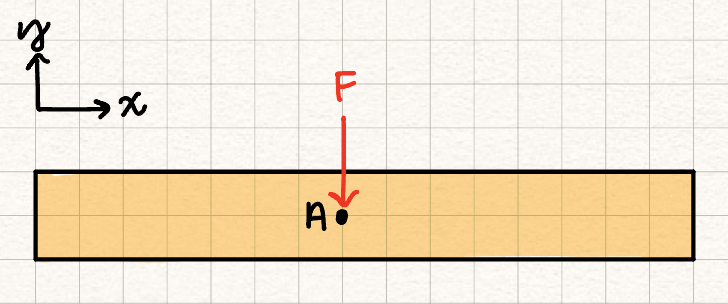
\includegraphics[angle=0, width=5 in]{ForceSystemsFigures/ConcentratedForce.PNG}
\vspace{-2mm}
\caption{\small A concentrated force applied to a bar at point A.}
\vspace{-3mm}
\label{Fig:ConcLoad}
\end{figure*}

\subsection{Distributed loads}
%from lecture 11 and 12

Distributed loads (usually written as $w(x)$) are forces applied over a length, volume, or area. The SI units for distributed loads are N/m. These loads, written as a function of length $x$ can be simplified into an equivalent force, $F_R$, which results in the same external loading on the rigid body. 

The magnitude of the equivalent force $F_R$ is the area under the $w(x)$ curve. The location of the resultant force $F_R$ is the location of the centroid of the shape of the force curve. 

\blue{Later, we can add a side comment about examples of distributed loads in real life. For example, books on a bookshelf, air pressure over a lake, the distribution of loads on on the ground over your foot when you take a step}

\subsubsection{Rectangular loading}

For a constant distributed load of magnitude c applied to a bar over a length l, the resultant force magnitude is 

\[F_R = c*l\]

the resultant force location is at $l/2$.

\begin{figure*}[!h]
\centering
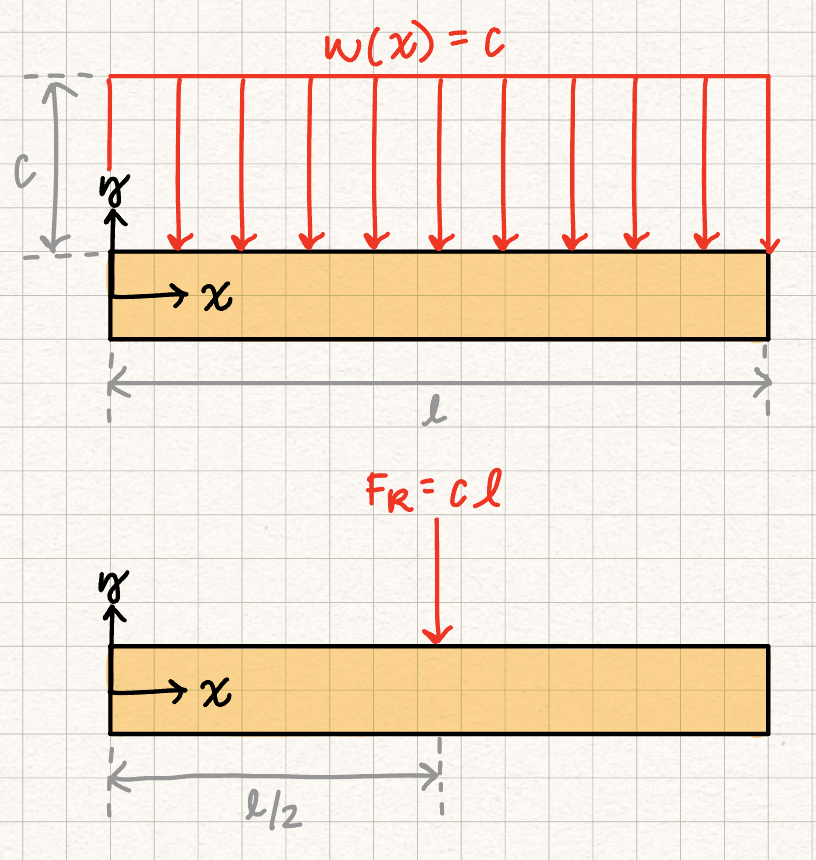
\includegraphics[angle=0, width=5 in]{ForceSystemsFigures/DistLoad.PNG}
\vspace{-2mm}
\caption{\small Example distributed load (top) and its equivalent force system (bottom).}
\vspace{-3mm}
\label{Fig:DistLoad}
\end{figure*}


\subsubsection{Triangular loading}

For a triangular distributed load (a uniformly varying load), the magnitude of the load is equivalent to the area of the triangle. 

\[F_R = 0.5*c*l\]

The location of $F_R$ is 1/3 from the base of the triangle. 


\begin{figure*}[!h]
\centering
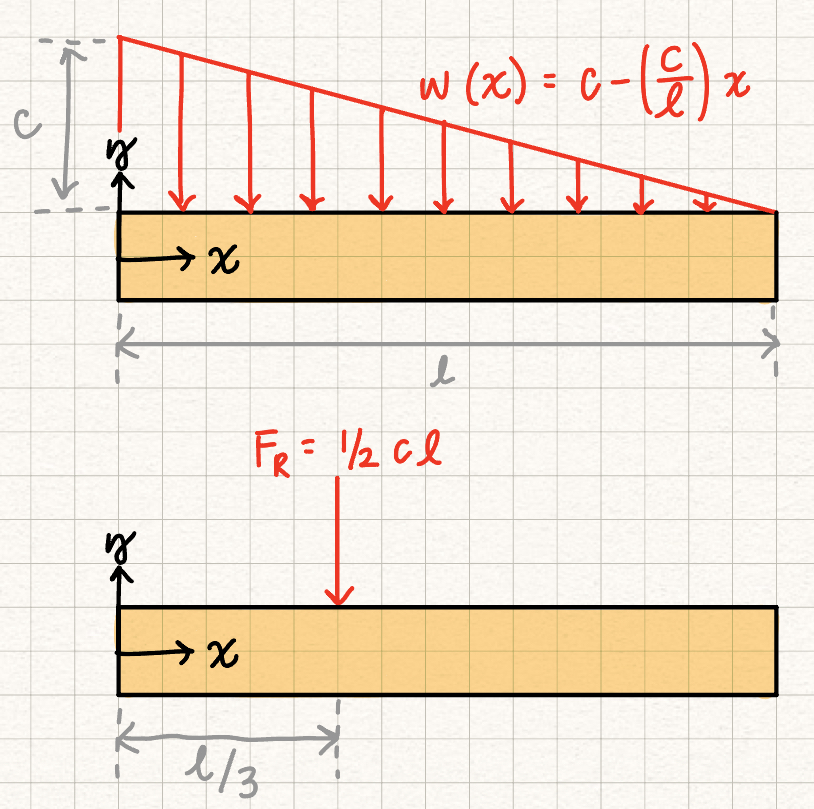
\includegraphics[angle=0, width=5 in]{ForceSystemsFigures/TriangleLoad.PNG}
\vspace{-2mm}
\caption{\small Example triangular distributed load (top) and its equivalent force system (bottom).}
\vspace{-3mm}
\label{Fig:TriLoad}
\end{figure*}

%from lecture 11 and 12

\subsubsection{Nonuniform distributed loads}

More complex distributed loads can be reduced to two distributed loads of uniform shape, or the integral of the distributed load function can be taken to obtain the area under $w(x)$, which is $F_R$. 

\[F_R = \int_{0}^{L} w(x) \,dx \]

The location of $F_R$ on the beam can be found by solving for the moment $M_R$ about a point. In this case we will take the moment about the point $x$=0 and setting it equivalent to the moment produced by the resultant force $F_R$ at $x$=0. 

\[M_R = \int_{0}^{L} x*w(x) \,dx = \bar{x}*F_R\]

Now we can solve for the center of mass of the distributed load, $\bar{x}$, using

\[\bar{x} = \dfrac{M_R}{F_R}\]

\begin{figure*}[!h]
\centering
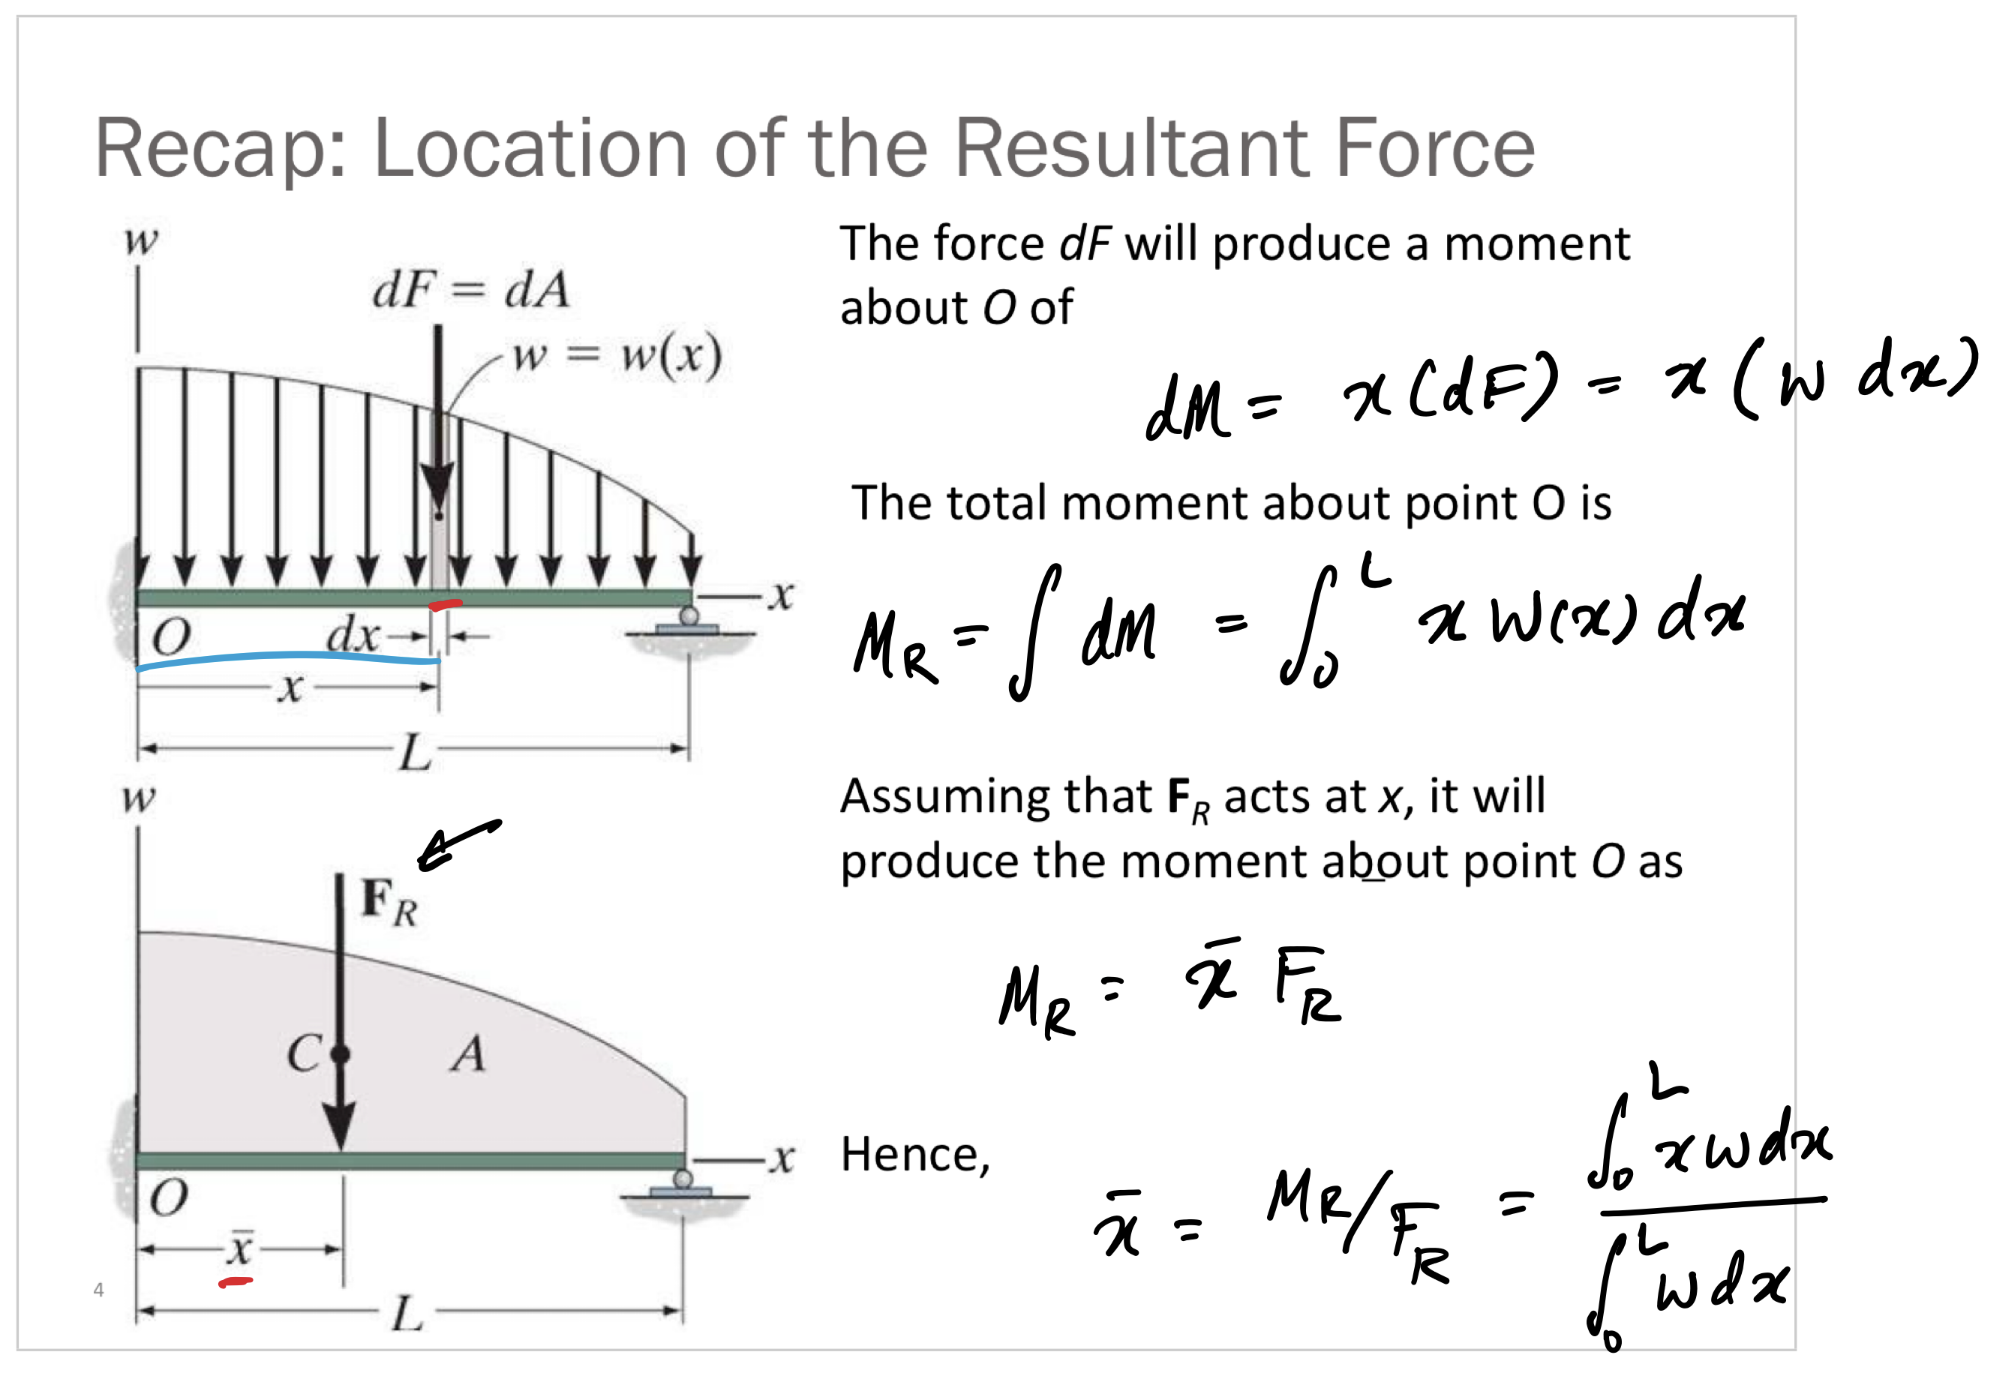
\includegraphics[angle=0, width=5 in]{ForceSystemsFigures/NonuniformLoad.PNG}
\vspace{-2mm}
\caption{\small Nonuniform load. Need to remake this in the same style as the other pictures.}
\vspace{-3mm}
\label{Fig:NonUniLoad}
\end{figure*}


%from lecture 11 and 12